% ADDED BY MATAN:	
\section{Reactive walking pattern generator}

\input{WalkingPatternGenerator}

\section{Regularization of contracting oscillators}
\label{sec:regularization_contracting_oscillators}

In this section we will use the work done by M. Karklinsky and A. Mukovskiy and presented in \cite{matan:biorob:2016}.
For a given reference trajectory M. Karklinsky and A. Mukovskiy designed a contracting system using Andronov-Hopf oscillator.
The reference trajectory is a specific solution of the global dynamics. 
As a reminder, a dynamical system is contracting if all solutions in the contraction region converge exponentially to each other.
If a dynamical system is contracting, there exists an attractor in this contraction region, and all trajectories in the region converge exponentially to it \cite{lohmiller_contraction_1998}.
Contraction guarantees the exponential decays of
perturbations.
Partial contraction is contraction towards any of the particular solutions residing inside the flow-invariant manifold of the dynamics \cite{pham_stable_2007}.
For the current work, it suffices that the reference trajectory is an invariant one dimensional submanifold of partially contracting dynamics, with local contraction towards but not along the trajectory.
The partial contraction is easy to construct for an arbitrary trajectory, as demonstrated by M. Karklinsky and A. Mukovskiy in \cite{matan:biorob:2016} for cyclic trajectories.
Trajectories that are the natural test ground of power laws in human motion.
Each partially contracting system are regularized to obey a power law on all orbits, including the reference trajectory. 

\subsection{Morphed Andronov-Hopf oscillators}
This section recalls the construction of a stable dynamical system with desired limit cycle trajectory from an angular morphing of the basic Andronov-Hopf oscillator.

\subsubsection*{Angular morphed Andronov-Hopf oscillator}

The Andronov-Hopf oscillator \cite{park2009design}:
\begin{eqnarray}
\label{eq:angulardynamics}
\dot{\theta} &=& \omega\\ \nonumber
\dot{\rho} &=& \alpha(1-\rho)
\end{eqnarray}
With the winding angle $\theta$ and radius $r_0(\theta)$, defined as the orientation of the path's normal and its radius of curvature.
They are the direction and radius of the osculating circle as well.
$\rho=\frac{1}{r^2}=\frac{1}{x^2+y^2}$, $x,y$ being the Cartesian coordinates.
And with $\omega,\alpha>0$ being two constants.
For a path with positive (negative) curvature everywhere, like elliptic curves, the direction and radius of the osculating circle define $(\theta,r_0(\theta))$ at each point.
These coordinates on the path naturally extend to coordinates that cover a band around it.
For a constant $B = \min_\theta(r_0(\theta))-\epsilon>0$, in the compact band of width $B$ around the path, each point in the $(x,y)$ plane will map locally to one closest point with coordinates $(\theta,r_0)$.
Its coordinates will therefore be $(\theta,r(\theta))$; the winding angle and the distance from the center of the osculating circle of the closest point. 
To define a dynamical system on the angular coordinates, we define the coordinate $\rho(\theta) = \frac{1}{r^2(\theta)}=$, and use the dynamics from Eq.~\ref{eq:angulardynamics}.
It is partially contracting, since the Jacobian of the $\rho$ subsystem is uniformly negative definite $J_\rho<-\alpha<0$. 
This oscillator can be morphed \cite{ajallooeian_general_2013}:
\begin{eqnarray}
\label{eq:polarmorphingdynamics}
\dot{\theta} &=& \omega\\ \nonumber
\dot{\rho} &=& \alpha (F(\theta)-\rho) + \omega \frac{d F}{d \theta}
\end{eqnarray}
It is still partially contracting, with $F(\theta) = \frac{1}{r_0^2(\theta)} = \kap^2(\theta)$ the squared path curvature.
Global partial contraction in the $\theta,\rho$ coordinates to the limit cycle results in partial contraction to the reference path in the band of width $B$.

%%%%%%%%%%%%%%%%%%%%%%%%%%%%%%%%%%%%%%%%%%%%%%%%%%%%%%%%%%%%%%%%%%%%%%%%%%%%%%%%

\subsection{Temporal regularization of a dynamical system}

In this section, we define the power law regularization of dynamical systems and examine the conditions for its applicability. Under reasonable conditions, the regularized dynamical system has exponential convergence to the limit cycle of the original system. For some special cases the regularized system is contracting.

\subsubsection{Power law regularization}
We focus on regularization with a power law $\vv = \HH(\kap) = \gamma \kap^{-\beta}$, with $\gamma$ a global constant and $\beta$ the exponent value. This is the basic most useful example of the general Euclidean invariant dependency of speed upon path geometry, $\vv = \HH(\kap,\kaps,\dots,\kapn)$ (see \cite{bennequin_movement_2009}).

\begin{mydef} 
	For a dynamical system $\dot{\xnv} = F(\xnv)$, and a power law $\vv = \HH(\kap)$, we define the $\HH$-regularization of $F$, denoted by $\dot{\xnv} = F_\HH(\xnv)$, as $F_\HH(\xnv) = \frac{F(\xnv)}{|F(\xnv)|} \HH(\kap(\xnv))$, with $\kap$ the curvature of the orbit at point $\xnv$.
\end{mydef}
At each point, the orbit of $F_\HH$ geometrically coincides with the orbit of $F$. Additionally, the speed along each orbit of $F_\HH$ satisfies the law $\HH$.
Each velocity vector has the same direction in both system $F_\HH$ and $F$, but but not necessarily the same norm.
Our power laws are positively monotone so the directions of flows of $F$ and $F_\HH$ match. 

\begin{myass} We consider a region $U$ which is a compact trapping region in the plane for $F$ without fixed points. We require that for $F$'s orbits $\kap$ is defined and bounded, and therefore $\HH$ is defined and bounded; for each $\xnv \in U$, $\HH(\xnv)\geq C_1>0$ for some global constant $C_1$. We require that $F$ has bounded speed $|F(\xnv)|<C_2$ for some global constant $C_2$.
\end{myass}

These assumptions guarantee that, if $F$ is contracting in $U$ to some limit cycle, then each solution converges globally exponentially to this limit cycle in $U$ (see Lohmiller and Slotine's \cite{lohmiller_contraction_1998}, Theorem 1). While we do not claim that $F_\HH$ is generally contracting, our assumptions yield global exponential convergence of $F_\HH$ to the limit cycle of $F$. This is true because  $|F_\HH(\xnv)| = \frac{\HH(\xnv)}{|F(\xnv)|} |F(\xnv)| \geq \frac{C_1}{C_2}  |F(\xnv)|$. The limit cycle of $F_\HH$ is geometrically identical to that of $F$, and movement on it obeys the $\HH$ power law.






\subsubsection{Curvature of the orbits of the circular Andronov-Hopf oscillator}
Power law regularization has singularities in inflection points and along straight trajectories; if $\kap=0$ and $\beta>0$, the power law speed is infinite. This can be overcome in several ways. For most practical needs the power law speed $\vv$ can be bounded; Viviani and Stucchi \cite{viviani_biological_1992} defined $\vv = \gamma (\kap+\alpha)^{-\beta}$, with some constant $\alpha>0$ preventing the singularity at $\kap=0$. Alternatively, we can restrict the discussion to regions of positive curvature. For the morphed Andronov-Hopf oscillators, around a planned cyclic trajectory with positive curvature, there exists a band of bounded nonzero curvature, guaranteeing that the regularization process will result in finite speeds. 

The dynamics of $\rho(\theta)$ define $\kappa(\rho)$ along each orbit. For circular Andronov-Hopf oscillators, the dynamics are invariant with respect to rotations around the origin $(x,y)=0$. Therefore local curvature of the vector flow $\kappa(\rho)$ is a function of $\rho$ only, independent of $\theta$. For any integral trajectory its local curvature $\kappa(\rho)$ equals zero exactly where it crosses a circle $\rho_{\kappa=0}$ concentric to the unit limit cycle and bigger. Therefore, in the circular band $C\geq\rho\geq \rho_{\kappa=0}+\epsilon$, for arbitrarily small $\epsilon$ and arbitrarily large $C$, the curvature is strictly positive $\kappa\geq C_1>0$, speed is bounded, and our assumptions hold, allowing power law regularization that results in exponential convergence to the limit cycle. 


\subsubsection{A contracting one-third power law regularized elliptic oscillator }
For the one-third power law, any elliptic system generated as a linear transformation of the regularized unit circle oscillator is contracting. The argument of the unit circle regularized oscillator, based on the circular symmetry of $\kap$, holds for uniform scaling. A global equi-affine transformation of the plane conserves the one-third power law and therefore the transformation of the unit circle dynamics to elliptic dynamics using the combination of a scaling and an equi-affine transformation conserves contraction of the regularized system.
As a consequence a velocity vector field can be computed from any elliptic reference trajectory.
This velocity vector field has the property to make a point mass converge toward the reference trajectory if this point mass track the velocity of this vector field.
In Fig.~\ref{fig:ellipsis:power:laws} we can see the initial unit cycle oscillator in subFig.~\ref{fig:ellipsis:power:laws}.a.
This unit cycle can be morphed without loss of the contracting property of the reference trajectory (see subFig.~\ref{fig:ellipsis:power:laws}.b).
The subFig.~\ref{fig:ellipsis:power:laws}.c-\ref{fig:ellipsis:power:laws}.f correspond to the velocity vector field regularized by the power law with $\beta = -1/3,0,1/3,2/3$.
We can easily see here the influence of $\beta$ on the vector field.
If $\beta$ is small the velocity will be high when the curvature is high.

\begin{figure}[ht]
	\centering
        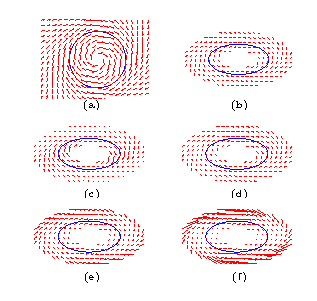
\includegraphics[trim=0.3cm 0.3cm 0.3cm 0.2cm,width=0.5\linewidth]{./figures/morphing.pdf}
	\caption{Morphing and regularization of an Andronov-Hopf oscillator. a)~The unit cycle oscillator. b)~an elliptic morphing. c)-f)~Four power law regularizations according to $\beta = -1/3,0,1/3,2/3$ power laws respectively. Each regularization keeps directions but changes speeds of the elliptic vector field.}
	\label{fig:ellipsis:power:laws}
\end{figure}


%%%%%%%%%%%%%%%%%%%%%%%%%%%%%%%%%%%%%%%%%%%%%%%%%%%%%%%%%%%%%%%%%%%%%%%%%%%%%%%%
\section{Results}
In order to evaluate the effect of applying the one-third power law to humanoid robot walking, we integrated the two third power law inside the Stack-of-Task framework. We present dynamic simulations and real robot experiments testing motions generated by the walking pattern generator (Fig.~\ref{fig:covertwothirdpowerlaw}). We compared four different power laws (Fig.~\ref{fig:ellipsis:power:laws}), with exponents $\beta=-1/3,0,1/3,2/3$. We explain the methodology and describe the results.

\begin{figure}[ht]
	\begin{center}
	  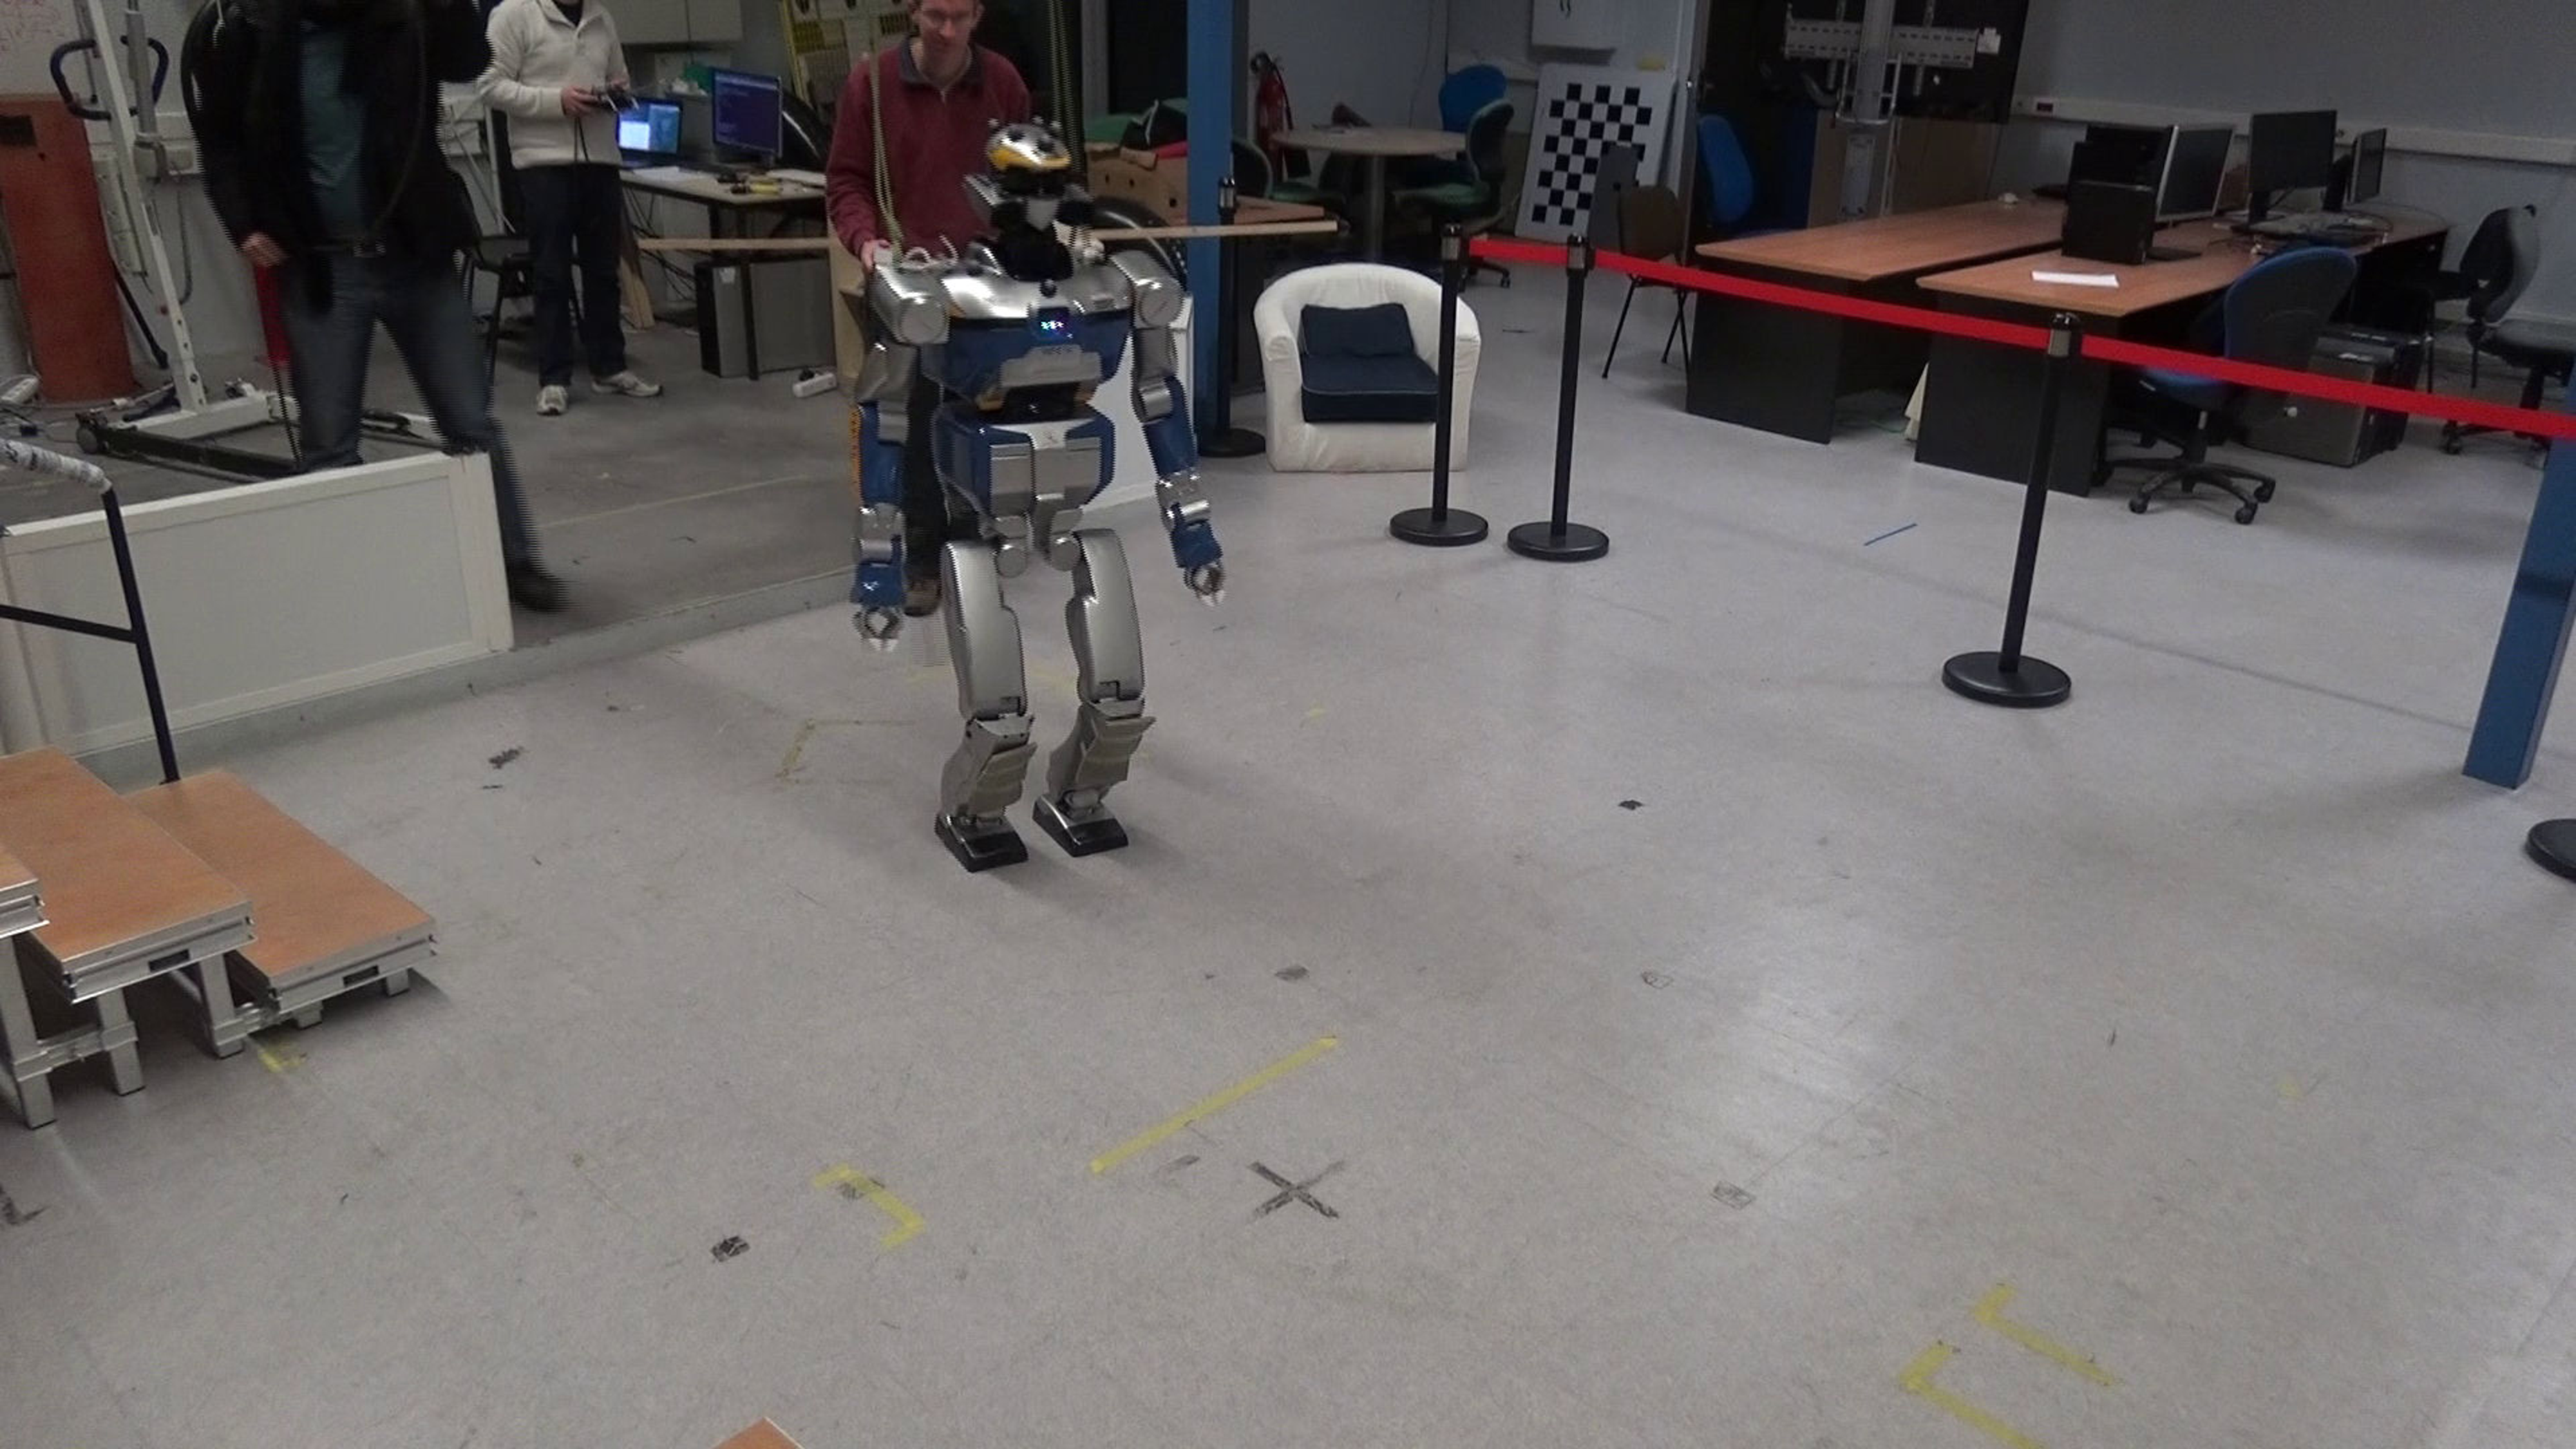
\includegraphics[height=0.25\linewidth]{./figures/RobotWalking.pdf} \hfill
	  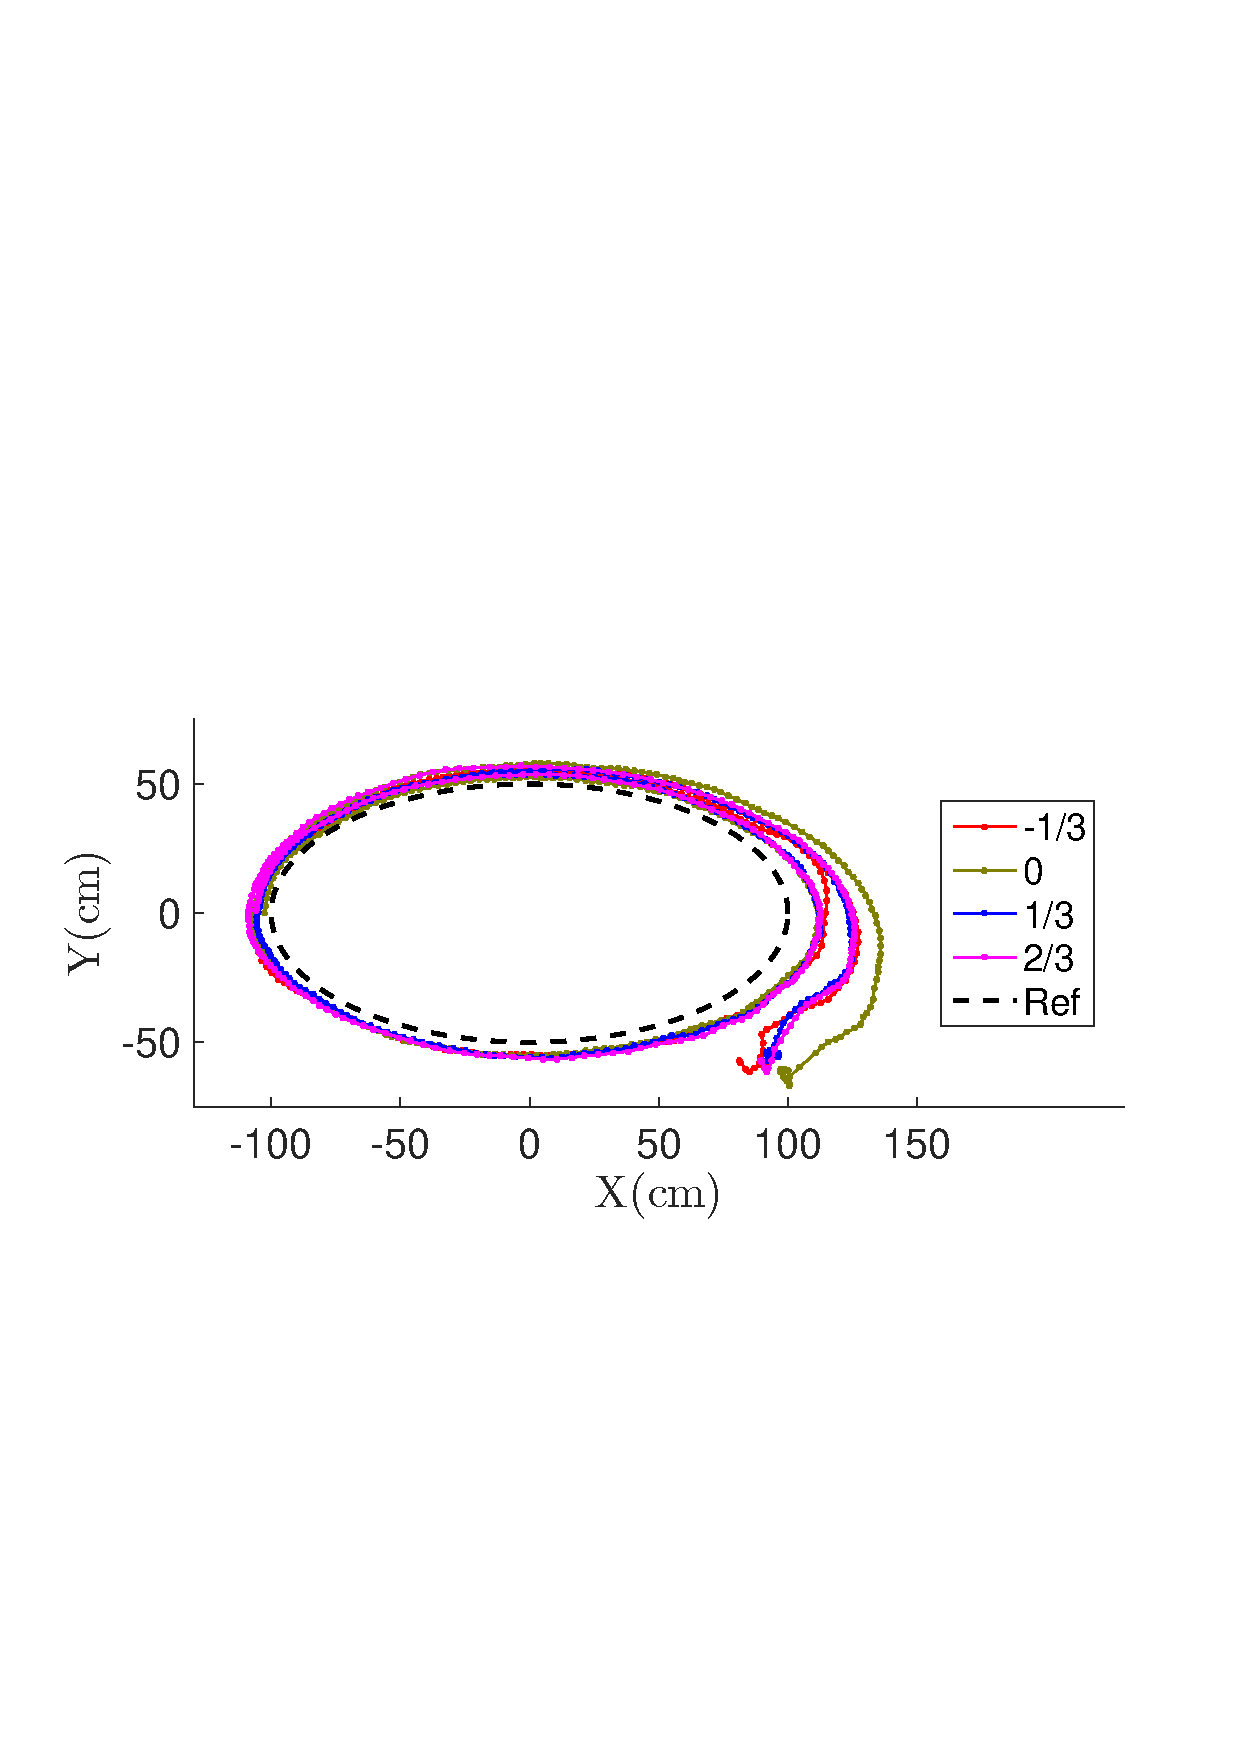
\includegraphics[trim=2cm 9cm 0cm 12cm,clip=true,height=0.25\linewidth] 
	    {./figures/Fig5d_EXPshapesSymmetric.pdf}
  \end{center}
	\caption{Experimental setup, the robot walks according to a reference ellipse, obeying one of four different power law speeds. Trajectories for each power law converge around a limit cycle ellipse. }
	\label{fig:5def}
\end{figure}

% NEW ANALYSIS,Simulation:
% Symmetric algorithm
%Beta: -0.33 |D: 27.22 |A: 1.8196 
%Beta: 0.00 |D: 8.96 |A: 1.6615 
%Beta: 0.33 |D: 0.05 |A: 1.5726 
%Beta: 0.67 |D: 0.13 |A: 1.5695 

% Durations:
% 140.0025
% 134.0025
% 130.0000
% 127.2000
% % Power law betas for both, using curvature of shape:
%DS:Beta O: -0.33 |LL: -0.21 |U: -0.21 
%EXP: Beta O: -0.33 |LL: -0.22 |U: -0.23 
%DS:Beta O: 0.00 |LL: 0.05 |U: 0.05 
%EXP: Beta O: 0.00 |LL: 0.02 |U: 0.02 
%DS:Beta O: 0.33 |LL: 0.33 |U: 0.33 
%EXP: Beta O: 0.33 |LL: 0.36 |U: 0.34 
%DS:Beta O: 0.67 |LL: 0.62 |U: 0.60 
%EXP: Beta O: 0.67 |LL: 0.63 |U: 0.57 
%% R squared (simulation, experiment)
%0.4599    0.7011
%0.2741    0.0318
%0.9905    0.7933
%0.9441    0.8953

%% With experiment sway removal - BAD FOR SPEEDS!
%DS:Beta O: -0.33 |LL: -0.21 |U: -0.21 
%EXP: Beta O: -0.33 |LL: -0.21 |U: -0.31 
%DS:Beta O: 0.00 |LL: 0.05 |U: 0.05 
%EXP: Beta O: 0.00 |LL: -0.05 |U: -0.12 
%DS:Beta O: 0.33 |LL: 0.33 |U: 0.33 
%EXP: Beta O: 0.33 |LL: 0.35 |U: 0.32 
%DS:Beta O: 0.67 |LL: 0.62 |U: 0.60 
%EXP: Beta O: 0.67 |LL: 0.68 |U: 0.67 
% r s
%0.4565    0.1097
%0.2720    0.0217
%0.9904    0.0994
%0.9443    0.2941
\begin{table}[h]	
	\centering % centering table
	\begin{tabular}{||c||cc|c|c|c||} % creating 5 columns
		\hline
		\hline
		SIM    &  &    & & &\\
		Ref.~$\beta$     & Sim.~$\beta$ & $R^2$   & MSD (cm$^2$)& A (m$^2$)&T (s)\\
		\hline
		$-0.33$ & $-0.21$ & $0.46$ & $27.22$  & $1.820$ & $140.0$ \\
		$0$     & $ 0.05$ & $0.27$ & $8.96$   & $1.661$ & $134.0$ \\ 
		\textcolor{red}{$0.33$}  & \textcolor{red}{$0.33$}  & \textcolor{red}{$0.99$} & \textcolor{red}{$0.05$}   & \textcolor{red}{$1.573$} & \textcolor{red}{$130.0$} \\
		$0.67$  & $0.60$  & $0.94$ & $0.13$   & $1.569$ & $127.2$ \\
		\hline
		\hline
		EXP     &  &    & & &\\		
		Ref.~$\beta$     & Exp.~$\beta$ & $R^2$   & MSD (cm$^2$)& A (m$^2$)&T (s)\\
		\hline
		$-0.33$ & $-0.23$ & $0.70$ & $53.13 $ & $1.888$ & $150.4$ \\
		$0$     & $ 0.02$ & $0.03$ & $30.51 $ & $1.812$ & $142.4$ \\
		\textcolor{red}{$0.33$}  & \textcolor{red}{$ 0.34$} & \textcolor{red}{$0.79$} & \textcolor{red}{$39.00$} & \textcolor{red}{$1.855$} & \textcolor{red}{$134.4$} \\
		$0.67$  & $ 0.57$ & $0.90$ & $46.11 $ & $1.884$ & $133.6$ \\
		\hline
		\hline
		REF    & $-$     &$-$     & $0$      & $1.571$ & $120.0$ \\
		\hline
		\hline
	\end{tabular}	
	\caption{Results from dynamic simulation (SIM) and actual robot experiment (EXP); for different reference power laws (Ref.~$\beta$), simulated power law exponent (Sim.~$\beta$) and actual motion power law exponent (Exp.~$\beta$) calculated using nonlinear regression \cite{maoz_noise_2005} with R squared error ($R^2$), mean squared distance to the reference path (MSD), area (A) and duration (T) of the generated ellipse trajectory are given, with those of the reference frame (REF). Geometrically, in simulation the one-third power law, $\beta=1/3$, is most exact, and in experiment the constant speed was more exact. Temporally, higher $\beta$ exponents yield faster  motions for both simulation and experiment, but always slower than the reference.}
	\label{table:dynamicsimulationsummary}
\end{table}
 % Experiment, cleaned with new
%Beta: -0.33 |D: 53.13 |A: 1.2020 | 
%Beta: 0.00 |D: 30.51 |A: 1.1538 | 
%Beta: 0.33 |D: 39.00 |A: 1.1812 | 
%Beta: 0.67 |D: 46.11 |A: 1.1999 | 
%1.8881
%1.8124
%1.8554
%1.8847


% EXPERIMENT, with one lap same as before
%MSD
%54.6913
%31.3508
%40.0416
%46.9112
%AREA
%1.8931
%1.8165
%1.8602
%1.8882

% Duration
% 150.3750
% 142.3925
% 134.3975
% 133.6125

% area (aaa)
%1.9454
%2.0069
%1.9272  * smallest!
%2.0018

% actual results for table
%msd (ddd)
%79.7895
%114.1826
%69.9704    * smallest
%87.6226

%%%%%%%%%%%%%%%%%%%%%%%%%%%%%%%%%%%%%%%%%%%%%%%%%%%%%%%%%%%%%%%%%%%%%%%%%%%%%%%%%%%%%%%%%%%%%
%%%%%%%%%%%%%%%%%%%%%%%%%%%%%%%%%%%%%%%%%%%%%%%%%%%%%%%%%%%%%%%%%%%%%%%%%%%%%%%%%%%%%%%%%%%%%
\subsection{Integration inside the Stack-of-Tasks framework}

Fig.~\ref{fig:covertwothirdpowerlaw} present the architecture of the system.
It shows that the "Vector Field" output is $\bf c^*$, but in fact the vector field only provides linear velocity assuming that the robot is heading forward.
Hence, inside the vector field box there is a Proportional Integrative Derivative (PID) controller which track the orientation of the velocity vector.
It tries to minimize the error $e=atan(\frac{\dot{y}}{\dot{x}}) - \theta$.
With $[\dot{x} \; \dot{y}]$ the linear velocity extracted from the vector field and $\theta$ the orientation of the robot base.
The singularities of the $atan$ function is dealt with inside the PID controller.

The control period of the HRP-2 robot is $5\,ms$.
$2\,ms$ are consumed by the walking pattern generator, $1\,ms$ by the QP solver and $1\,ms$ by the robot low level controller which includes the stabilizer.
The vector field has $1\,ms$ left to be computed.
Hence, in terms of computation time, we had to include efficient C++ code inside the Stack-of-Tasks.

\subsection{Dynamic simulation results}

\begin{figure}
	\centering
	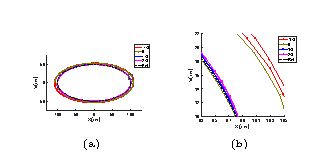
\includegraphics[trim=0cm 0.4cm 0cm 0.5cm,width=\linewidth]{./figures/dynamic_simulation.pdf}
	\caption{a)~Dynamic simulation paths, with different reference speeds. b)~Zoom in on the box in plot a. Simulations with positive $\beta = 1/3,2/3$ have no drift, less than $1$ cm from the reference path. Simulations with constant speed and negative power law $\beta = 0, -1/3$ drift outside of the reference elliptic path.}
	\label{fig:5ab}
\end{figure}


\subsubsection{Simulation and trajectory analysis}

To simulate motion, we used the OpenHRP simulator, that computes the contact forces and HRP-2's rigid body mechanics, and includes a model of the compliance of the robot ankles. We implemented the control architecture depicted in Fig.~\ref{fig:covertwothirdpowerlaw} in OpenHRP.
We analyzed the trajectories of the center of mass using MATLAB. To overcome the coronal swing motion we applied a procedure for finding the middle points of each sway. Each middle point was the average of two consecutive local signed curvature extrema with opposite signs, with time defined as the average of the times of these two points. We used the middle points trajectory for all analysis purposes. The values of the power law exponents $\beta$ were calculated using nonlinear regression estimation  \cite{maoz_noise_2005}. Repeating the procedure with $\log-\log$ linear regression yielded similar $\beta$ values. Speed was extracted from the middle points trajectory using a noise-insensitive filter \cite{Holobororodko2008}. Curvature was extracted from the reference ellipse.

\subsubsection{Power law patterns are reproduced}

The theoretical speed profiles are compared with the one measured in simulation (Fig.~\ref{fig:5g}, left) and the one measured from the motion capture system (Fig.~\ref{fig:5g}, right).
The simulation yielded positions of maximal speed slightly shifted with respect to maximal speed positions predicted by the power law based on the curvature of the actual path; for $\beta=-1/3,1/3,2/3$ shifts along the trajectory, of $22,4,-15$ cm of the simulated with respect to reference speed peaks occurred.
Unpredictably, constant speed $\beta=0$ power law yielded an oscillatory curvature-dependent speed profile. 
% OLD simulation:
% Beta: -0.33 |D: 0.22 
% Beta: 0.00 |D: 0.97 
% Beta: 0.33 |D: 0.04 
% Beta: 0.67 |D: -0.15 

\subsubsection{Drift correction by one-third power law}
As predicted, the simulated one-third power law resulted in reduced drift compared to constant speed and other power laws. For $\beta=1/3$ the path was most similar to the reference path, with next best being the $\beta=2/3$ power law. The constant speed $\beta=0$ and $\beta=-1/3$ yielded drifts; the simulated elliptic paths were larger than the reference elliptic path, as reflected by area and mean squared distance (see table \ref{table:dynamicsimulationsummary} and Fig.~\ref{fig:5ab}). Interestingly, the constant speed $\beta=0$ path deviated from the reference frame gradually and not immediately upon movement initiation, as seen in  Fig.~\ref{fig:5ab}.b.


\subsubsection{Increase in $\beta$ exponent decreases duration}
Simulated motions took more time than the reference time, that was always two minutes per lap. The power law exponent affected movement duration; the higher the $\beta$ the faster the motion, so its duration was closer to the reference behavior (table \ref{table:dynamicsimulationsummary}).


\begin{figure}[ht]
	\centering
	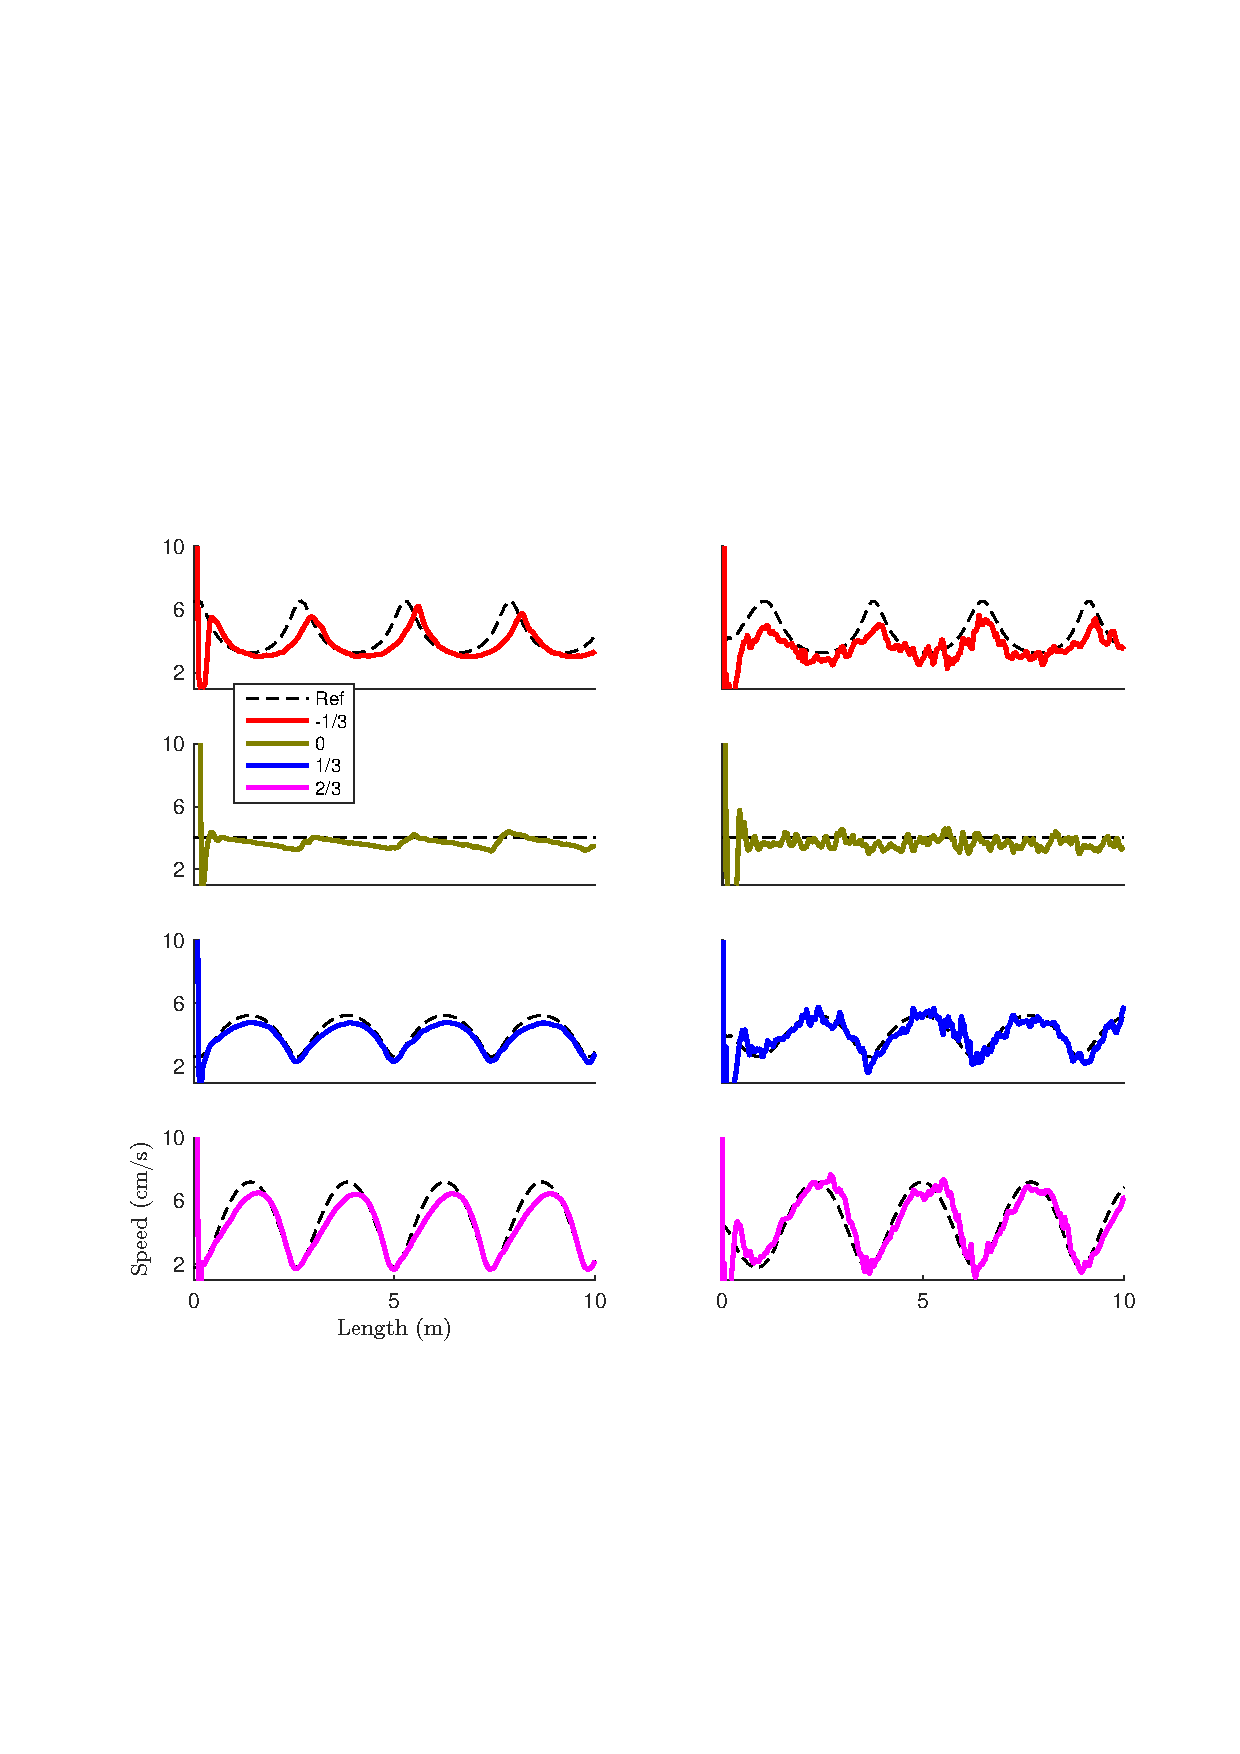
\includegraphics[trim=2cm 7cm 1cm 9.1cm, clip=true,keepaspectratio,width=0.8\linewidth]{./figures/Fig5g_DSspeedprofilesBoth.pdf}
	\caption{Speed profiles for dynamic simulations (Left) and robot experiment (Right), with four different reference speeds (Ref). Both simulated and actual robot motions reproduce the spatio-temporal power law patterns.}
	\label{fig:5g}
\end{figure}

% OLD: Simulation only
%\begin{figure}
%	\centering
%	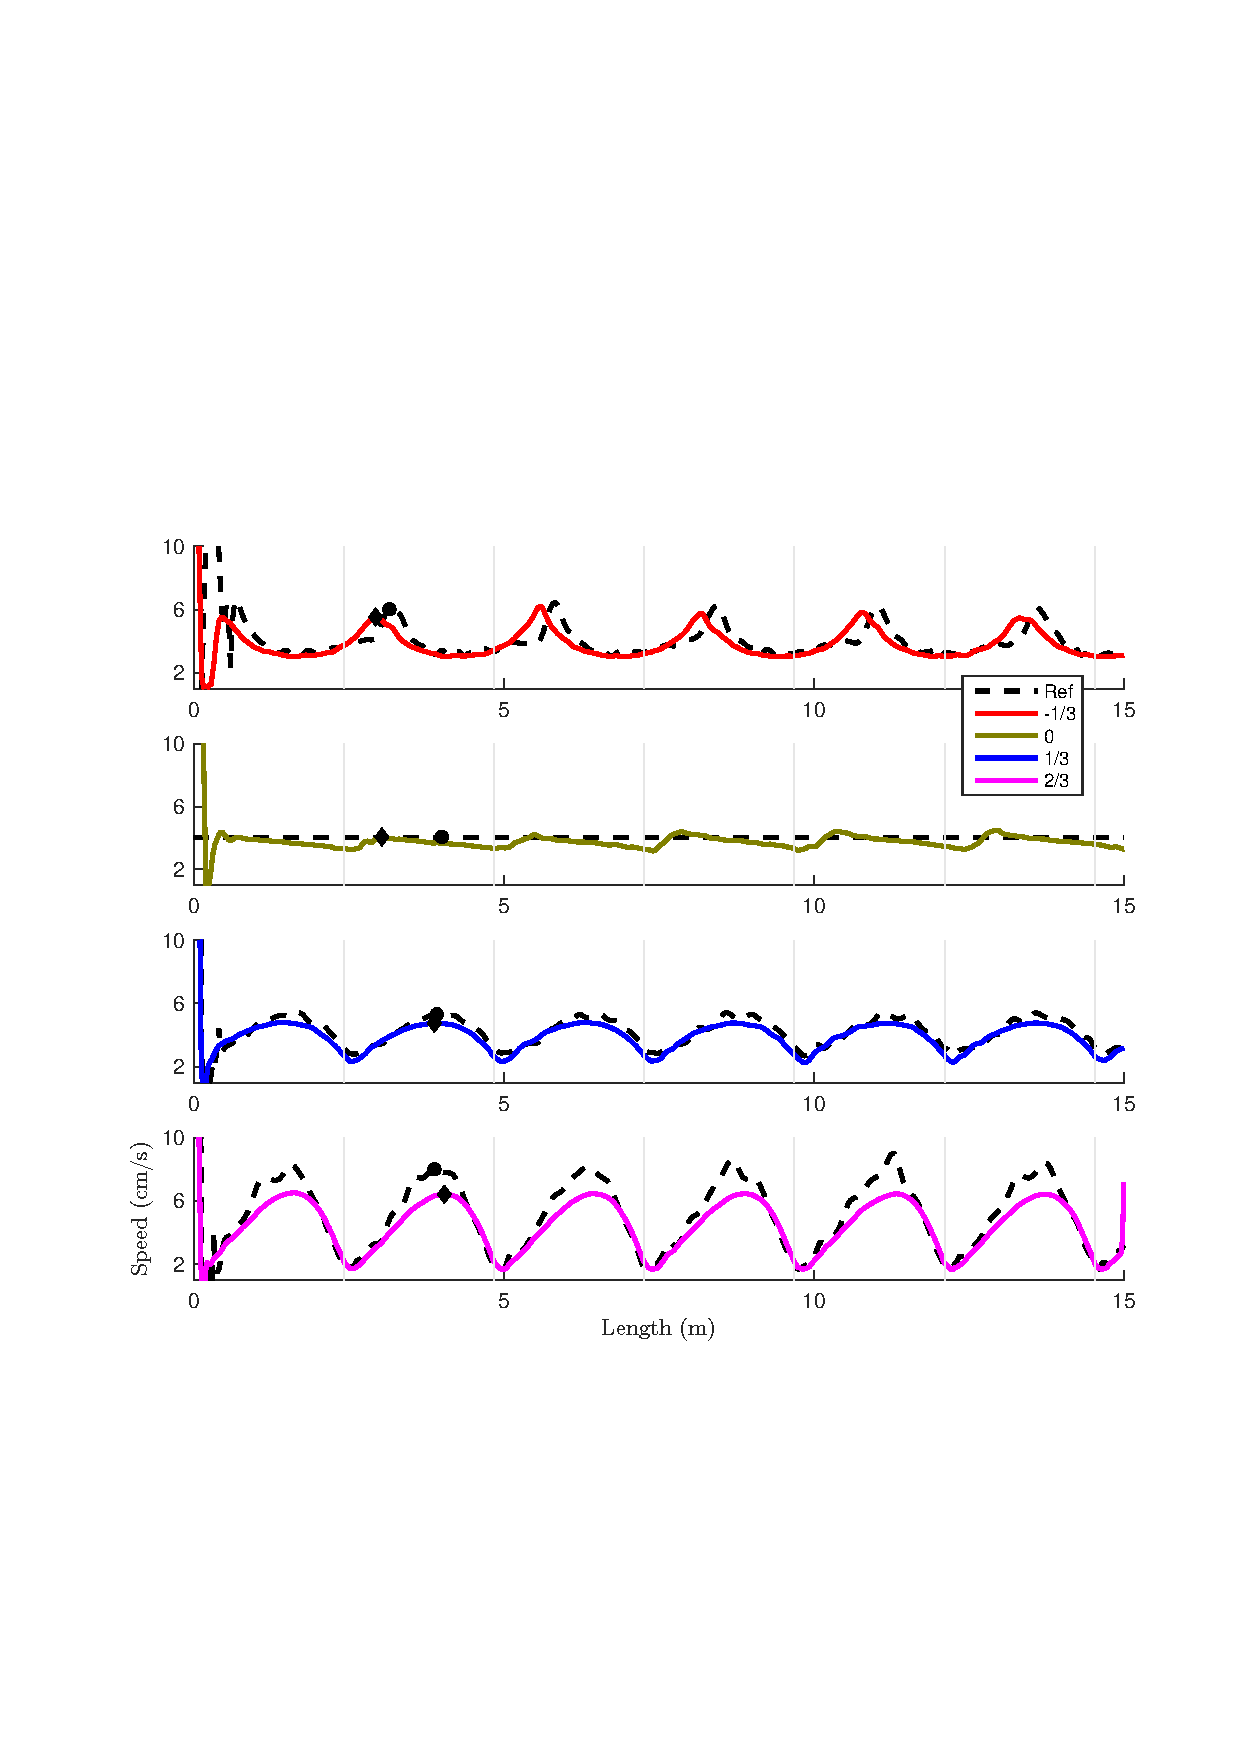
\includegraphics[trim=2cm 7cm 2cm 9.1cm, clip=true,keepaspectratio,width=1\linewidth]{./figures/Fig5c_DSspeedprofilesSymmetric}
%	\caption{Dynamic simulation with different reference speeds (Ref). Only for $\beta=1/3$ the simulation matches reference speed. Constant reference speed simulation slows near planned curvature maxima (perpendicular gray lines). The locations of speed maxima of the simulated trajectory ($\blacklozenge$) and reference trajectory ($\bullet$) for $\beta=1/3$, differed by a $4$ cm distance, less than for $\beta=-1/3,\beta=2/3$, that had more than $15$ cm distances. We calculated reference speeds using curvature of the actual path.}
%	\label{fig:5c}
%\end{figure}


%%%%%%%%%%%%%%%%%%%%%%%%%%%%%%%%%%%%%%%%%%%%%%%%%%%%%%%%%%%%%%%%%%%%%%%%%%%%%%%%%%%%%%%%%%%%%
%%%%%%%%%%%%%%%%%%%%%%%%%%%%%%%%%%%%%%%%%%%%%%%%%%%%%%%%%%%%%%%%%%%%%%%%%%%%%%%%%%%%%%%%%%%%%

\subsection{Experimental results}
\subsubsection{Experimental setup and trajectory analysis}
We tested the four power laws with the actual HRP-2 robot; the robot started standing approximately $60$ cm behind the tip of the ellipse, and walked until completing two laps. We used center of mass trajectories measured with the motion capture system, low pass filtered at $0.1$ Hz.  Analysis was identical to that of simulated motion.  


\subsubsection{Power law patterns are reproduced}
The reference speed power laws were noisily reproduced by the robot (see table \ref{table:dynamicsimulationsummary} for $\beta$ values and their $R^2$ errors, and figure \ref{fig:5g} for speed profiles). 

\subsubsection{Geometrical drift does not fully vanish}
Overall, experimental results showed larger drifts than simulation. The constant reference speed resulted in the lowest drift (table \ref{table:dynamicsimulationsummary}), outperforming the positive $\beta$ power laws. Different convergence trajectories (see figure \ref{fig:5def}), may arise from different initial positioning. 
 
\subsubsection{Increased $\beta$ decreases duration}
The actual movement of the robot took longer time than simulation. The trend we reported for the simulations; the higher the $\beta$ the faster the motion, was fully reproduced in the experiment.

\subsubsection{Evaluating controller corrections}

\begin{table}[ht]
	\centering 
	\begin{tabular}{|| c || c | c | c | c ||c |} 
		\hline 
		\hline 
		Ref.~$\beta$        & $-0.33$  & $0$      & \textcolor{red}{$0.33$} & $0.67$   \\
		\hline  
		Norm     (m)        & $1.416$  & $0.950$  & \textcolor{red}{$0.642$} & $1.124$ \\   
		Orientation (deg)   & $76.83$  & $89.60$  & \textcolor{red}{$60.45$} & $77.28$ \\ 
		Force ($kN\times$s) & $21.93 $ & $23.54$  & \textcolor{red}{$19.80$} &$21.01$  \\ 
		\hline
		\hline 		  
	\end{tabular}
	\caption{Analysis of the odometry frame and forces. For each of the four power laws the distance from center (Norm), body orientation (Orientation) and integrated norm tangential force measured on ankle (Force) are given. The one-third power law is outperforming all other power laws.}
	\label{tab:odometry_drift}
	
\end{table}

To estimate the  feedback correction done by the vector field and the PID controllers, we analyzed the internal odometry frame of the walking pattern generator. For each reference power law we examine the last crossing point of center of mass trajectory with the $x$ axis. We measured deviation from the baseline, the planned position and orientation, to gain error values reflecting the accumulated error along the two laps, caused by sliding . Additionally we examined tangential forces on the ankle, indicating the amount of compensated sliding. The one-third power law showed smaller accumulated errors, compared to the other power laws (table \ref{tab:odometry_drift}). Less error needing compensation implicates lower burden on the hardware.
 
%\begin{table}[h]
%  \centering 
%  \begin{tabular}{|| c || c | c | c | c |} \hline 
%    $\beta$     & -1/3    & 0.0    & 1/3    & 2/3    \\ \hline  
%    Norm        & 1.416   & 0.950  & 0.642  & 1.124  \\ \hline  
%    Orientation & 76.83   & 89.598 & 60.453 & 77.217 \\ \hline 
%  \end{tabular}
%  \label{tab:odometry_drift}
%\end{table}


\section{Conclusions}

In simulation and experiment, we tested how stable generation of power laws may help humanoid robot walking. 
The simulations and experiments reproduced the reference power law's temporal patterns.
The one-third power law, used by humans, appears beneficial for drift reduction. The one-third power law reduced drift in simulations and also resulted in less need for sliding compensation in actual robot motion.
Finally, our simulations and experiments showed that using higher $\beta$ exponent power laws allows faster movements. 

Having shown the importance of using a path-adjusted speed profile, it is still not fully determined how to select an optimal speed profile for stabilized and accurate robotic locomotion, given a planned reference trajectory. The different perspectives describing how the human motor system selects movement speed, based on either optimization \cite{flash_coordination_1985,todorov_optimal_2002} or geometric invariance \cite{flash_affine_2007,bennequin_movement_2009}, may prove beneficial for this aim. 

%To fully clarify the contribution of specific temporal patterns to different facets of human and humanoid locomotion is left for future studies.

%\subsection{From center of mass regulation to full body locomotion}
%Extending the regularities of a specific trajectory and forming globally converging dynamics is required to stably generate humanoid motion. Section \ref{sec:regularization_contracting_oscillators} addressed two issues. First, building a regulator around a given reference trajectory, is needed for spatial drift compensation during trajectory execution. Second, power law regularization allows transforming the temporal structure of a trajectory to a pace regulator on the plane. A systematic examination of these two processes is called for. Interestingly, defining the center of mass behavior is just the beginning. One example has to do with the necessity of contact switching from one footstep to another. In the current study, the time between footsteps was fixed and speed was realized by modifying the step length. However, freely determining contact times may improve the quality of the trajectory tracking.  
Except for systematic examination in locomotion of the benefits of different speed regularities, we suggest two additional applications of the speed modulation according to the geometry of the reference trajectory. One is to use power laws as a constraint for kino-dynamic motion planning  \cite{Pham:rss:2009}, the other is to find bounds on curvature when planning the motion of the free-flyer \cite{Orthey:PhD:2015}. 

%The pattern generator used in this system is the predominant source of constraints which do not allow perfect tracking of the guiding trajectory. 


%In this study, all the constraints are either purely mechanical or motivated by the
%control one-third power law, as they are the constraints formulated in the optimization problem solved for walking.
%The evident benefit for humanoid motion of the one-third power law may be based upon deep characteristic properties that are common to the two legged motion of both humans and humanoids. Finding these properties is left for future work.


%\subsection{}
%[] Containing: Problems, analyze them, extensions]
%\begin{itemize}
%	\item Why is 2/3 power law better?
%	\item Problem of 
%
%\end{itemize}

%\subsection{Dynamical systems for generation of robust cyclic behavior}
%
%\subsection{Temporal and geometrical aspects of the }
%\subsection{Regularization of dynamical systems}
%[XXX put here or in the methods?]
%The process of power law regularization, which we applied on the morphed Andronov-Hopf oscillators, is a specific instance of a more general process of speed regularization. For an arbitrary dynamical system and an arbitrary regularity law of motion, determining how speed is dependent on geometry of trajectories, the regularization process is applicable wherever $H$ is well defined. Wherever the original dynamics converge and the regularity law is monotone (a curve parametrization with no zero speed), the regularized dynamics are also converging. If the original dynamics are exponentially converging and the change of speed induced by the regularization is bounded then the regularized dynamics are also exponential. This happens if the original system is contracting, but also in other cases. A natural question is what conditions guarantee that a regularization law conserves contraction, namely transforms an original contracting system to a regularized contraction system. We have proven that the one-third power law regularization of an area-preserving morphing [XXX equi-affine?] of the basic Andronov-Hopf oscillator, this is the case. 
%
%[XXX Tamar: do you think we should omit this or keep?]
%Power laws in general, and specifically the one-third power law, can not describe movement through inflection points, as predicted speed goes to infinity. This drawback was resolved by the work of Bennequin et al. \cite{bennequin_movement_2009} which incorporated Euclidean, equi-affine and full-affine geometries in the mixed geometries model, to account for movement speeds along general trajectories. The regularization process proposed here is easily extendable to a mixed-geometry regularization process. 
%
%Another alternative description of movement speed along a desired trajectory is 
%  
%
%\subsection{Coordinate systems for convergence to a trajectory}
%
%\subsection{From center of mass trajectories to multiple dimensions}